\documentclass{iitkthesis}

\begin{document}

\title{Dialog-Based Wayfinding Using Intrinsic and Extrinsic Attributes of Landmarks}

\author{Arbaz Khan}
\iitbdegree{Master of Technology}
\department{Computer Science and Engineering}
\rollnum{Y9227128}
\setguide{Prof Harish Karnick}
\setguidedept{Computer Science and Engineering}
\setcoguide{Prof Bharat Lohani}
\setexguide{Prof. Stephan Winter}
\setcoguidedept{Department of Geoinformatics}
\setexguidedept{Department of Geomatics}
\setexguideaff{University of Melbourne}
\dissertation
\maketitle
\makecertificate
\begin{abstract}
Using landmarks in communicating routes leads to a more natural 
navigation concept for humans as compared to simple turn-based 
instructions. Modern day navigation assistance services use name-based 
reference for landmarks in route instructions, which are not always 
recognized by a wayfinder (due to his unfamiliarity with such references).
Moreover, these rely on an interface for communicating routes which 
requires support for web connectivity, graphics rendering and location 
sensing in the end-device. In this work, we propose a model for dialog-based 
navigation assistance for localization and route guidance using visual 
and geometric characteristics of landmarks. We discuss a localization 
algorithm based on speed prediction for estimating the location to 
facilitate incremental route guidance. We also consider the issue of 
disorientation and provide strategies for reorienting a lost person. 
Further, we evaluate the model for quality of service by assisting 
artificial agents in navigation using synthetic datasets of landmark 
attributes.
%We also provide an insight into the complexity of the untackled problem of resolving the frame of reference.
\end{abstract}
\tableofcontents
\chapter{Introduction}
\section{Problem Statement}
The goal of this thesis is conceptualization, implementation and evaluation of a model for navigation assistance which relies upon the geometric and visual characteristics of landmarks to localize and guide a person from a known source to a known destination using spoken-dialog interactions as the interface.
\section{Notions and Terminology}
\subsection{Wayfinding}
Human wayfinding is the process of purposeful and directed movement from 
an origin to a specific destination. It is different from spatial 
exploration, the other form of navigation where 
the goal is not to reach a specific destination but to contribute to 
cognitive map formation of an environment. So the daily trips that a 
person makes to his work-place from his home is a wayfinding task, while 
exploring an unfamiliar neighborhood in the town is locomotion or 
exploration. The problem of wayfinding is: identify the ordered 
sequence of actions that must be performed in a spatial environment to reach 
a desired location. For a car driver in a street network, these set of 
actions are related to determining the turning behaviour at every 
intersection that he encounters. For a person in a museum looking for a 
specific art form, these set of actions would be a sequence of hallways 
he needs to walk through, to get to the intended location. 

Further, it is easy to see that in our everyday interaction with space 
we are often involved in wayfinding tasks. In some, the exact sequence of 
actions is very familiar but in 
others we need either external assistance or a personal strategy to 
find the way. The former requires acquisition of spatial knowledge 
of the environment either through prior experience or through static 
information learned from maps and/or other media-based resources (and so 
is prone to errors). Similarly, personal strategies used in wayfinding do 
not guarantee success in reaching the destination. Traditionally, 
people have used maps,sketches and compasses as external tools for 
wayfinding. These guidance instruments have evolved over the years to 
mobile navigation systems as the need was to provide incremental 
instructions as the person moves in space. This has 
proved more effective as the information on what needs to be known 
is provided only when needed. This approach shapes the 
modern form of assistance - \textit{location-aware} wayfinding. 
\subsection{Location Awareness}
A service is said to be \textit{location aware} if it allows a user to 
discover and communicate his position in the real world using some  
form of external hardware support. Location awareness has become 
a key component in many mobile computing applications \cite{parctab}. 
In the context of navigation, we can say that if the end-device knows it's 
geographical location the service is location-aware. This definition 
comes from the realm of location-aware computing where location-awareness 
means ability to provide services based on the geographical location of a 
mobile device. Primarily, there are three different techniques for 
location sensing - Triangulation, Scene Analysis and Proximity Sensing 
\cite{hightower}. In modern location-aware services, GPS (a form of triangulation) is the 
most widely used because of it's better relative accuracy as compared to other known techniques. 
The Invisible Ideas Project \cite{perry} was the first of it's kind to use macromedia flash and GPS 
technology to provide location-aware services.

It is easy to see how location-awareness can help in way-finding. 
With the help of techniques for location-awareness, a mobile device is
able to determine it's geographical location using sensing technology (such as GPS) 
and then relay this information (along with any identity-based data like 
user ID, device ID, etc.) to the service provider. Thus, it can be a platform 
for realizing an effective wayfinding assistance system which can provide 
incremental delivery of instructions to the user based on the location of 
the user. 

\subsection{Landmarks}
A \textit{landmark} is a salient and distinguishing feature of it's spatial environment. Landmarks are primarily used in navigation as reference points for confirming orientation and identifying actions at intersections \cite{lovelace}. Any spatial object qualifies as a landmark if it is distinctly different from it's surrounding.  The distinctiveness is defined w.r.t attributes of the landmark. Based on the representation of a landmark in a relational model, the attributes of the spatial features can be divided into four categories:
\begin{itemize}
  \item \textbf{identitificational} - these attributes include \textit{reference-id} as a pointer to the spatial feature, and \textit{category} specifying the class of the spatial feature. The values to category attribute can come directly from the data to which they belong (e.g., \textit{buildings} and \textit{parks} are stored seperately).
  \item \textbf{geometric} - for a spatial 2-D database, geometry comes as a primitive datatype representing the structure in coordinate space. This allows the definition of functions to handle geometry based operations and provide mathematically derived attributes such as area, length.
  \item \textbf{visual} -  these attributes define the visual characteristics e.g., height of a building\footnote{It is assumed that the spatial data available uniformly across the world is 2-D and hence, height does not fall under geometric attributes.}, color of a structure.
  \item \textbf{semantic} - these attributes are defined as per external sources and are meant to identify the meaning or purpose behind a feature e.g., petrol-pump, ATM.  The major attribute that falls in this category is \textit{popularity} of the feature as a landmark which facilitates context-aware wayfinding.
\end{itemize}

While the first feature is dependent on the data organization, visual and geometric attributes can be defined to be \textit{intrinsic} attributes as these are present or can be easily extracted from exisiting spatial databases\footnote{From the visual attributes defined in \cite{raubal}, \textit{shape} and \textit{fa\c{c}ade area} can be completely extracted from spatial databases using geometric attributes, while \textit{color} information is extracted from laser scanning and complete \textit{visibility} analysis requires 3-D representation.} Semantic attributes are \textit{extrinsic} attributes, as these are not inherent characteristics of a feature and external resources (such as crowdsourcing or yellow pages) need to be used for their extraction.
\section{Background}
Modern advancements in technology have diminished the diffiulty 
in discovering and implementing wayfinding strategies. With the 
advent of smartphones, it is possible to build powerful 
applications which can show maps and compute routes based on preferences. 
It has removed the inconvenience of carrying a map and understanding it's 
symbols and notation. The navigation services are dynamic, that is the 
representation of graphical information keeps changing with respect to 
the current information about the user. This is where location-awareness 
comes into the picture and applications have utilized the power of this 
facility to customize their functionality to maximally benefit the users. 
The quality of user experience has evolved over a series of developments 
with offerings like 3-D representation of the environment showing up 
places nearby for better orientation. Significant effort has been put 
into the research and development of systems for navigational 
assistance. With the techniques of augmented reality, it has been now 
made possible to attach digital information (such as images, voice notes) 
to the environment. Furthermore, local information on weather and traffic 
has been incorporated into these applications to further enhance an 
interactive wayfinding environment.

%{For ineffectiveness of GPS, refer to PLace Lab}
Despite the powerful services offered by digital navigational aids, there 
are some problems as well. When a service is location aware, 
the end-device needs to have typically high processing speeds to process 
communicated information. Apart from 
the installation and usage costs associated with these services, the 
limited accuracy of these positioning systems is a vital concern. The 
inaccuracies extend from measurement errors in positioning systems from 
satellites to those in the map-matching algorithms \cite{white2000} that 
attempt to associate recorded GPS data points\footnote{These associations 
are unreliable to an extent and usually mismatch in dense street networks 
with diverging roadways, overpasses and underpasses} with the correct 
roadway. The GPS sensors suffer from poor service coverage and need clear 
vision to the sky to allow location locking. Thus, GPS limitations extend 
to subways, underpasses, indoor environments and dense street networks 
with tall buildings. Furthermore, deploying a location sensor like GPS 
has overheads of cost and power consumption.

The other limitation associated with modern day wayfinding services is 
their utter dependence on the extrinsic information for providing route 
assistance. The quality of route instructions are based upon the details 
in the map and the available landmark information through crowdsourced 
databases. This availability is fairly non-uniform and the success in 
providing utility is highly variable. it's easy to find regions where the 
route instructions in these commercial applications have no incorporation 
of existing landmarks (due to their unrecorded entry in the spatial 
databases), and are merely turn-based. Also, despite the availability of 
the landmark information does not guarantee good quality route 
instructions unless the representational names used are consistent and 
recognised universally or locally. For example, since not all streets in 
India have names, various popular mapping services and applications which 
rely upon street names to convey route instructions, had to invent their 
own street naming conventions and thus are observably ineffective in the 
context of navigation assistance.

Beyond these limitations, most of the services require an internet 
connection between the server and the client particularly for 
delivering map data or route based information. Streaming such  
information requires good internet connectivity. Storing offline maps is 
an alternative option but may not be always feasible.   

\section{Motivation}
A pure voice-based way-finding cum location-tracking 
model would eliminate the high-end device requirement. Here we discuss two
major reasons for such a way-finding model. 
\subsection{Why design a dialog-based system?}
In addition to the above shortcomings in modern digital navigation 
services, research \cite{jensen2010,dalton,reagan2006} has 
identified user preference for auditory assistance as well as a memory 
advantage for auditory over visual information. It has been observed 
\cite{baldwin2009,furukawa2004} that auditory guidance facilitates the 
task of way-finding whereas visual guidance facilitates cognitive map 
formation. Ego-centeric auditory instructions (i.e., based on the driver'
s perception) reduce the workload in navigation for drivers who are 
involved more in the task of route learning rather than cognitive map 
formation. Besides this, a graphical interface is likely to seriously 
interfere with driving while talking or listening on a hands-free mobile 
device is less intrusive. Wayfinding 
can be treated as one of those tasks that demand high level of attention 
to avoid any road-side risks. Auditory route instructions have been 
observed to be processed and followed without interference to the driving 
task \cite{jensen2010,dalton}.

Experiments \cite{srinivasaneffect} have also indicated an additional 
benefit associated with auditory guidance. The reaction times are 
faster with pure auditory route instructions compared to electronic 
route maps or turn-by-turn displays. 

Furthermore,  one major advantage of a dialog system 
is that context-identification can be implemented by studying the 
response of the user to the instructions/questions. This helps in 
personalising the service to navigational 
strategies preferred by a user. Most navigation assistance 
technologies are still visually dominated and the use of audio has been 
little researched. In the literature we have not found any comparable research 
that has exploited the usefulness of plain voice dialog for 
navigation purposes.
\subsection{Why choose to be location-unaware?}
Most end user mobile devices (typically cell phones)  in India are low cost 
vanilla voice phones that also be used for texting. They do not have a GPS or
other location sensors.

%Also, it has been suggested in research \cite{itsbarry} that in a joint activity where there is a coordination to achieve a private/personal goal, spoken dialog interactions are more effective than typed conversations and has been put to use in designing intelligent tutoring systems. This indication serves a clue that reading out the route instructions should be more effective as compared to text-based communication. 

 \section{Objectives of the work}
We target the design of a \textit{Dialog-based, location unaware way-finding
} model which exploits the auditory mode of route guidance and eliminates 
the need for global positioning systems. A service is location-unaware if 
the end-device has no location sensitivity and can not determine it's 
physical location either by itself (e.g.,GPS) or by sensing the resources 
from the environment (e.g., Infrared or wireless media). To further 
define a \textit{location-unaware} service, we describe it as a service 
under a pseudo location-aware model where one can determine the 
location of the end-user only approximately within a certain tolerance
without employing any location identification hardware support from the 
end-user device (in our case a cell phone). 

In this thesis we have conceptualized, designed and implemented
{
\textit{a dialog-based way-finding system with pseudo location-awareness.}
}

More concretely, the objectives are:

First, to communicate route instructions, we have designed a cross-lingual way-finding platform which gives instructional output in a simple
formal language. This formal language can be easily translated to
any natural language using a natural language generation module.

Second, we use a dialog based approach that uses intrinsic and extrinsic attributes of 
landmarks to localize a user during the entire way-finding session.

Third, we aim to minimize the dependence of the system on any extrinsic 
information. By extrinsic information, we mean any information that is 
not readily and uniformly available due to the needs of large-scale 
manual processing e.g., crowdsourcing, or database built from a place 
directory/gazeteer (gazeteers are not available for all places). The 
intention is to maximize the use of inherent characteristics of an 
environment like the height and color of buildings, the existence of an 
open space and hence it's shape, surrounding vegetation, etc. Such 
characteristics can be automically extracted from standard detection 
systems like LIDAR.

Fourth, we plan to provide a pure speech-based service which demands 
nothing more than an auditory medium for communicating with the mobile end-
user. Thus, the service functions independent of 
support for any wireless technology (such as bluetooth) or web access.
  \section{Roadmap}
Our design for way-finding uses dialog-based conversations to localize a 
user and guide him to the destination. To make the model generic, we design 
a communication protocol based on a formal representation of route instructions
to convey the path to the destination. The algorithm generates
a structured interaction for tracking the user's 
location in terms of en-route landmarks encountered. 
\textit{Chapter 3} introduces the semantics of this communication protocol. It also discusses the system architecture of a generic dialog-based wayfinding model, the key modules of which are elaborated throughout this thesis specific to a location-unaware realization.
In \textit{Chapter 4}, we present the localization algorithm to determine user's location by generating prompts for location tracking. It also discusses on the strategy adopted to reorient a user disoriented from his path due to possible misinterpretation of route instructions or because of an erroneous behaviour. 
\textit{Chapter 5} discusses the key implementation-specific aspects of the model which was used to study the effectiveness of the algorithm. These are related to building the knowledge-base underlying the proposed model and, implementing reorientation strategies for a lost person. 
To evaluate `goodness' of the algorithm, a simulation platform was set up to model a user with homogenous and non-homogenous speed patterns and erroneous behaviour in following the route instructions. \textit{Chapter 6} elaborates upon the employed simulation setup describing the user-modelling and a synthetic dataset of landmark attributes. We also introduce the goodness metrics used for evaluating the quality of service of the route guidance model. We end in \textit{Chapter 7} by providing a brief summary of the contributions made by the work and an outlook on possible improvements of the model. 

 \chapter{Related Work}
 \section{Dialog Based Wayfinding Systems} 
Significant research has been done in the area of defining 
\cite{lovelace} and generating \cite{Dale,Habel,Maab,pattabhiraman} good 
quality route instructions which are specialized for human understanding. 
These models have evolved from those working on handcrafted data 
disseminating turn-by-turn instructions in a one-step-per-sentence 
mapping to the systems processing data from Geographic Information 
Systems (GIS) using visible features of the surroundings and generating 
compact and more human-like descriptions. Yet, most of these systems were 
one-way systems in which the instructions are provided in advance or 
even incrementally leading to poor comprehension and 
an inability to resolve ambiguities along the path. Owing to the 
benefits of a dialog system to respond to user queries and the possibility to 
react to inadequate or poorly understood instructions, research  
\cite{hurtig, jokinen, richter} had moved towards building dialog-driven 
wayfinding models. The major concern in these systems is to avoid 
overwhelming the user with too much information (or media) to avoid cognitive 
overload while giving enough detail to produce comprehensive and accurate 
descriptions preventing any ambiguities or confusions. Some \cite{richter} 
of these systems rely on purely speech-based interaction while others 
\cite{hurtig,jokinen} have used a multimodal interface which offers the user 
freedom to combine speech, pen and graphics based input. 
Although, multimodal systems do help a user to choose the preferred mode of
interaction and consequently result in better and disambiguated input signals
they compromise the main requirement of wayfinding assistance, which is, to 
reduce distractions while driving. 
Pure-auditory based route instructions help in minimizing the 
interference to driving and thus create no negative impact on reaction 
times \cite{srinivasaneffect}. 
 
At present, there are very few systems using just spoken 
dialogue for wayfinding. These systems can be classified into 
three categories depending on the target domain - indoor wayfinding, human
-machine interaction and outdoor wayfinding. The systems \cite{fongsurvey} 
based on human-machine interaction aim to facilitate the machine in 
execution of spatial tasks by providing route information and handling 
questions raised on detecting ambiguities. These tasks though 
certainly are similar to real world wayfinding assistance models in 
dialog structure and end goals but differ in the ability of their subjects. 
Humans follow subjective and non-uniform speed-patterns, instruction 
understanding behavior and conceptual memory models. 

For outdoor wayfinding, Janarthanam et. al. \cite{janarthanam} introduced 
a mobile dialogue application that combines GIS systems with spoken-
dialog to assist tourists in city navigation. It allows 
tourists to initiate tasks such as entity search (e.g. a museum or a 
restaurant), navigation assistance, entity inquiry and others. The 
proposed architecture is capable of fairly complex spoken-
dialog interaction (e.g., Take me to Hume) with the help of it's semantic 
parser and  modules for natural language generation (NLG) and 
understanding (NLU). Richter et. al. \cite{richter} worked on generating 
context-based route instructions for outdoor wayfinding. Using a spoken 
dialog interface, the proposed conceptual model allows a user to tune the 
details of the route instructions from incremental turn-by-turn 
instructions to a more abstract set of instructions focussing upon 
destination descriptions. The model identifies and adapts to the wayfinder's 
spatial knowledge about the street network after deciding the prominence 
of a spatial entity derived from a hierarchy of visual, structural and 
cognitive features. Spoken-dialog systems for indoor wayfinding systems 
have not been built so far to the best of our knowledge. Cuay\'{a}huitl 
et. al.  \cite{heriberto} worked on a text-based dialogue system for indoor 
wayfinding which can respond to user queries on locations in a building. 
The authors claimed that a dialogue system for indoor wayfinding with 
only text-based interaction leads to very high overall scores of user 
satisfaction. Despite the fact that indoor settings are perfect for 
application of location-unawareness, yet none of these systems have  
attempted it and rely on certain location sensitivity (such as support 
for infrared and wireless media) in the end-device. Also, the relatively 
less emphasis on evolution of pure spoken-dialog systems can be 
understood owing to their limitations in poor speech recognition and 
unfulfilled linguistic expectations. 

In this work we try to overcome these limitations by setting up a cross-
lingual communication platform to convey non-ambiguous route instructions.
Furthermore, questions posed to the user for location tracking are 
such that the responses are recognisable speech commands 
(such as `yes',`no') and require only primitive speech processing. 
 \section{Evaluation Techniques}
Simulations in a virtual environment provide an important means for 
evaluation and improvement of real-world systems. Once the virtual 
environment is set-up, the next task is to identify the metrics for 
evaluating effectivenss of the system. The work done in this thesis is 
closely related to natural language generation (NLG), except that we focus 
only on the spatiotemporal content of the expressions. Thus, the 
technique and metrics used for evaluating NLG systems are relevant in 
this context. For example, if the number of users who reach the target 
are fewer, it reflects poorly on the quality of the NLG and thus 
could be related to the underlying spatio-temporal content of the 
instructions. It is only recently that increasing effort has 
been put into evaluation of NLG systems. As Spanger et. al. \cite{spanger} 
point out, there can be two categories of methods to evaluate the 
effectiveness of an NLG system - intrinsic and extrinsic. \textit{
Intrinsic} methods compare the system with a benchmark/gold standard 
system, and \textit{extrinsic} methods use metrics like the number of 
mistakes made by the user while following the instructions \cite{young}. 

Further, research on evaluation of NLG tasks and investigation of issues 
has moved towards introducing shared task challenges \cite{give}. In this 
task the evaluation is assessed based on the performance of human users 
who follow the instructions of the NLG in a virtual environment with 
several rooms and corridors. The performance evaluation uses a set of 
objective as well as subjective measures. Objective measures include the 
distance travelled and time taken in reaching the goal as well as the 
number of instructions provided and the number of words per instruction. 
While, subjective measures provide a subjective rating of these 
instructions whether the instructions were useful. An interesting area of 
research \cite{GRUVE} then emerged which works on modelling navigation 
assistance with real world problems like uncertainty in location and 
noisy feedback signals from the user. These works exploit the utility of a 
virtual environment to eliminate the time and costs of real world 
experiments as well as provide a means to manipulate the environment 
targeting specific issues and context.

In this work, we move beyond the above mentioned virtual environments 
tested on humans. With the virtualization of the spatial environment, we also 
virtualize the user via driver modelling and use a set of goodness 
metrics to measure the effectiveness of the system. Independent works 
have been done in the area of simulating driver behavior to study traffic 
and accident patterns but none of these have been integrated into a 
testbed for wayfinding assistance.

%Since, in our case where no gold standard system is available and directly comparing the sytem to GPS would be unfair
%Simulations in a virtual environment provide an important means for evaluation and improvement of real-world systems.  
 %Performance evaluation on a task is the basic requirement to measure effectiveness of a natural language generation (NLG) system \cite{reiter}.  
 \chapter{Conceptual Model For Wayfinding}
 \label{chap:concept}
We introduce our location-unaware wayfinding model through a generic 
spoken-dialog based model for wayfinding. This model can be transformed 
to a location-unaware wayfinding model by specializing the module 
structure. The aim of this model is to assist wayfinding tasks using 
natural language dialogues. The next section presents an architecture of 
the model. We propose a natural language independent communication 
protocol for conveying route-instructions.
 \section{Architecture}
The generic wayfinding model is designed to incorporate any linguistic 
structure and a predefined technique for user localization. It could 
be personalized for an user and should be able to identify and react to 
the context realizing the differences and constraints. The knowledge base 
behind is dynamically updateable to incorporate 
the changes in the spatial environment (such as broken road links, new 
buildings, etc). An architecture for the system realizing the requirements is 
shown in Figure \ref{fig:arc}. 
 \begin{figure}
\centering
%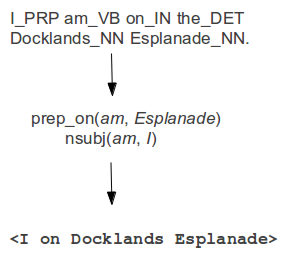
\includegraphics[width=0.5\textwidth]{phase1.png}
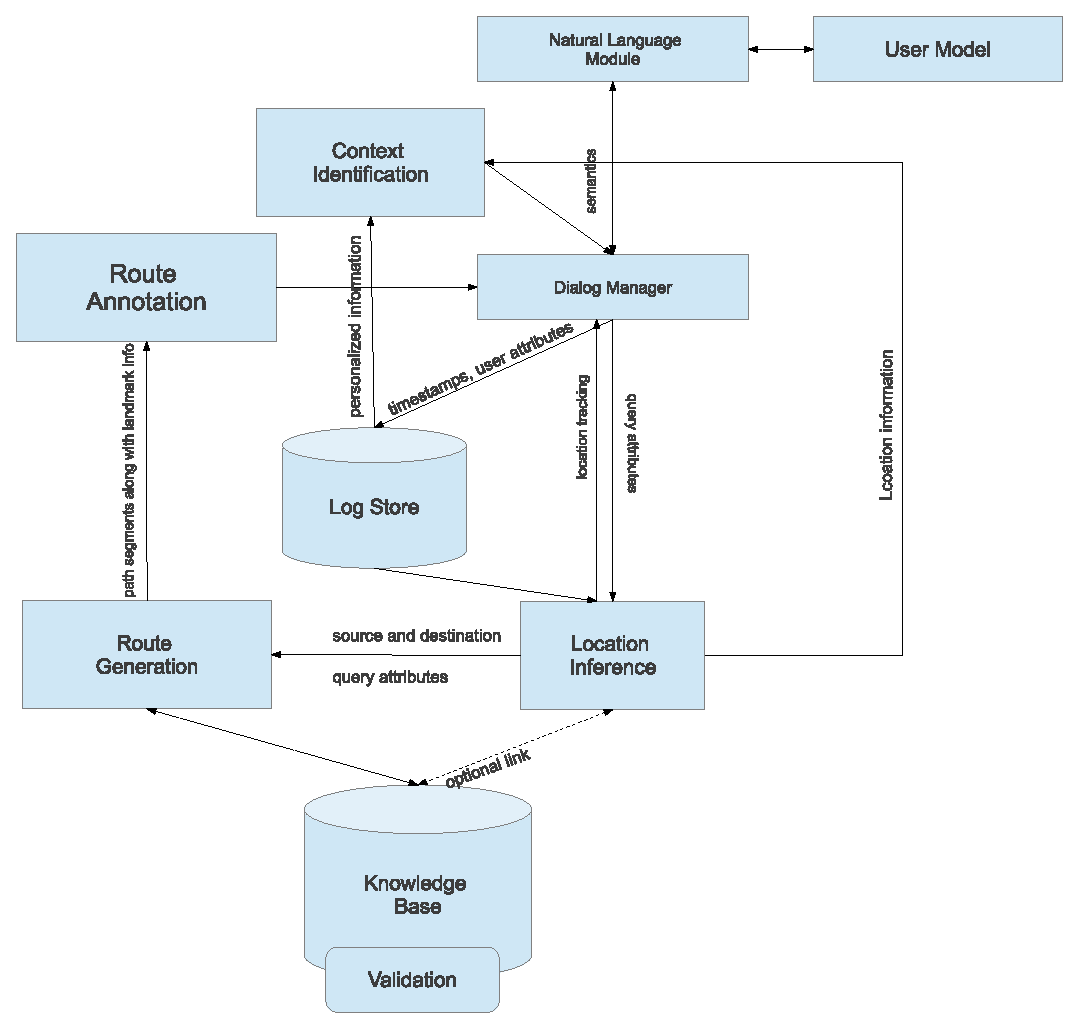
\epsfig{file=architecture.eps, height=4.2in, width=4.5in}
\caption{Architecture for a generic wayfinding model}
\label{fig:arc}
 \end{figure}
First, a \textit{user} (real human or artificial agent) requests for assistance 
to a destination. The \textit{Natural Language Module} parses the 
semantics of utterances, processes spatial information and records a new 
query into the system. Before route instructions are generated, it 
is necessary to locate the user (obtain the source location). Most of the 
wayfinding systems today use GPS systems for this purpose in an outdoor 
environment and wireless or infrared in indoor settings. Baus et. 
al. \cite{baus} introduced an adaptive model for localization that 
alternates between the different sensing technologies to overcome their 
individual limitations. For our system, we seek 
the user's location via dialog-based tracking, posing simple questions 
using features of a spatial environment. Nonetheless, we can abstract a 
module specifically for \textit{location inference} which either can work 
independently (by using sensors or receptors) or use the 
\textit{knowledge base} of the system for localization. Thus, the 
knowledge base stores a characterization of the complete spatial 
environment. It also stores the transportation network for target modalities 
(e.g., road links for vehicles, abstract spaces for pedestrians) and it's 
relationship with the environment features (e.g., landmark-street 
association).

Once the information required to compute the topological route is 
collected, then the desired route is computed using query attributes 
(such as preferred route option like shortest route, scenic route, etc. 
and modality constraints like roads permissible for 4-wheelers). This 
computed route is passed on together with nearby landmark information for 
\textit{route annotation}. The route annotator processes the salience of 
the landmarks, removes redundant spatial relationships and fills up the 
spatial content of the route instructions. Besides operating on the 
processed information, the system is also sensitive to the context i.e. 
user attributes (such as modality, speed patterns) and location 
information. The context needs to be considered before generating natural 
language route instructions. With the help of contextual information, a 
decision is made by the \textit{dialog manager} on the delivery of route 
instructions to synchronize with when a user needs it. So, 
decisions like these make sure that turn instructions are temporally 
matched with an user's movement. The dialog manager also compiles the route 
instructions into a form understandable by the natural language module, 
which then serves to eventually fulfill the user request.
  \section{Communication Protocol}
In this section we introduce a communication protocol which allows
cross-lingual platform development. The protocol is targeted to deal with 
two kinds of scenarios - simple intersections and complex intersections. 
These latter scenarios deal with intersections having a 
large number of possible actions (more than 4) and tackling 
ineffectiveness of standard direction models. In similar 
work, Klippel \cite{klippel} introduced a formal representation of turn 
directions at decision points which could be chunked to produce better 
quality route instructions and could be tailored as per user preferences. 
But the formal theory model targets only simple intersections. Our 
approach is based on a similar notational representation of turn 
instructions but extends to complex intersections as well. The goals in 
designing this protocol are: 
\begin{enumerate}
\item \textbf{Completeness}
The protocol should indicate the action to be taken at each decision 
point implicitly or explicitly. A set of good quality instructions avoids 
the need to specify the action at each decision point by chunking action 
behaviour. For example, instructions `\textit{go straight}' and 
‘take a left turn’ can be compactly presented as ‘take the second left 
turn’ which implicitly directs action behaviour at each decision point 
and is arguably more comprehensible. 
\item \textbf{Non-ambiguity}
An ambiguous language model leads to confusion in the action required at each 
decision point and could lead to disorientation. For instance, 
instructing to take a left turn in a topology as shown in Figure 
\ref{fig:turnA} is ambiguous and it is not sure whether to take a left at 
$e$ or $f$.
\item \textbf{Applicability}
Alongwith completeness and non-ambiguity, it is equally important to 
consider the ease of applying the communication protocol in a real-world 
scenario. This means that the protocol should be structured such that it 
could be translated easily to the desired natural language.
\end{enumerate}
 \begin{figure}
\centering
%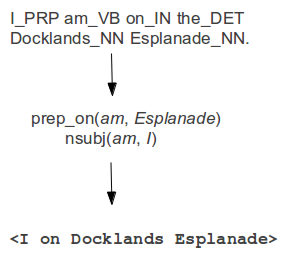
\includegraphics[width=0.5\textwidth]{phase1.png}
\epsfig{file=turnA.eps, height=1.5in, width=1in}
\caption{Ambiguity arises when the route instructions are based on 
standard direction models as \textit{take a left}.}
\label{fig:turnA}
 \end{figure}

 \begin{figure}[htb]
\centering
%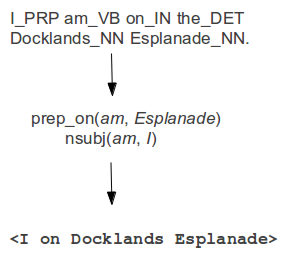
\includegraphics[width=0.5\textwidth]{phase1.png}
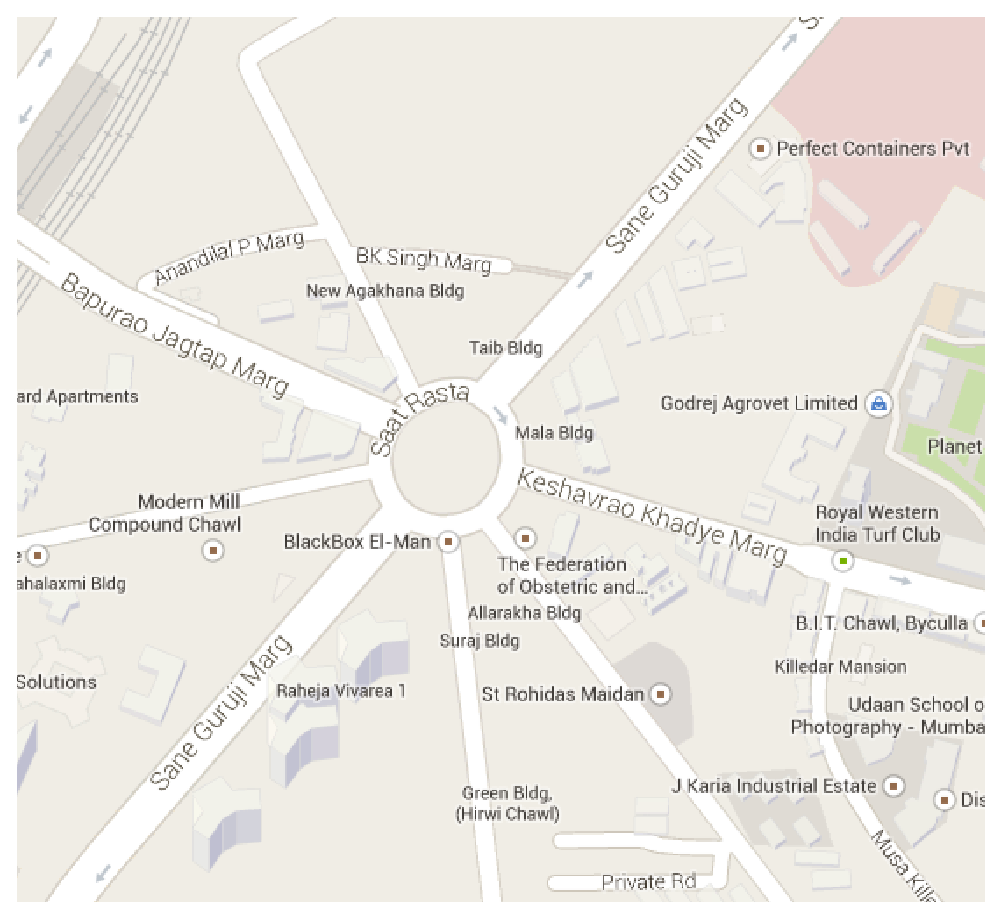
\epsfig{file=complex_real.eps, height=3in, width=3in}
\caption{Real world example of a complex intersection in Mumbai, India 
taken from Google Maps \cite{gmaps}.}
\label{fig:complex_real}
 \end{figure}

The communication protocol proposed is an adaptive approach to formal 
representation of route instructions. It uses a standard direction model 
similar to Klippel \cite{klippel} when the resulting indications are non-ambiguous. However, if the turns are complex, it uses a clock-based 
convention to represent turn directions. The protocol uses a language 
independent symbolic encoding for landmarks and turn instructions at 
decision points. The two scenarios of simple and complex intersections 
differ in the symbolic encoding of directions while landmarks use their own 
notational representation and below we elaborate on each of these. 

\subsection{Landmarks}
The landmarks are represented by notational IDs and by the direction 
(left or right) in which an user encounters this landmark while moving on 
a path segment. So, if $X$ is the notational ID of a landmark and if 
moving on the directed path segment, the user would encounter $X$ on his 
right, then the corresponding representation is $X^R$. Similarly, $X^L$ 
indicates that moving on the path segment, user can see $X$ on his left. 
These representations along with that of turn behaviour at intersections 
(simple and complex) form the communication protocol. 

\subsection{Simple Intersections}
Most of the intersections in the real-world fall under this category and 
are fairly trivial to communicate. To formally define a \textit{simple 
intersection}, we divide field-view of the navigator in four triangular 
zones (see Figure \ref{fig:simpleturns}). Choosing reference axis as the 
left direction perpendicular to the incoming road segment $p$, the left 
zone spans 45 degrees on either side of the reference point. it's mirror 
image in the field-view w.r.t. the decision point is the right zone. 
Similarly, one can conceptualize the other two zones. We define a 
decision point as a \textit{simple intersection}, if in each zone of the 
navigator's field view, there is atmost one road segment emerging from 
the decision point. 

The instructions that are associated with change in direction are 
represented by symbols \textbf{R} and \textbf{L}. The non-turning 
instruction indicating that one should go straight is represented by {\bf S}. 

\begin{figure}
\centering
%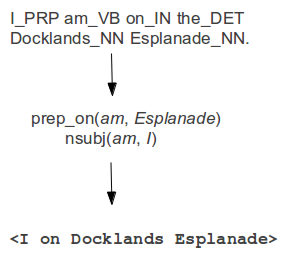
\includegraphics[width=0.5\textwidth]{phase1.png}
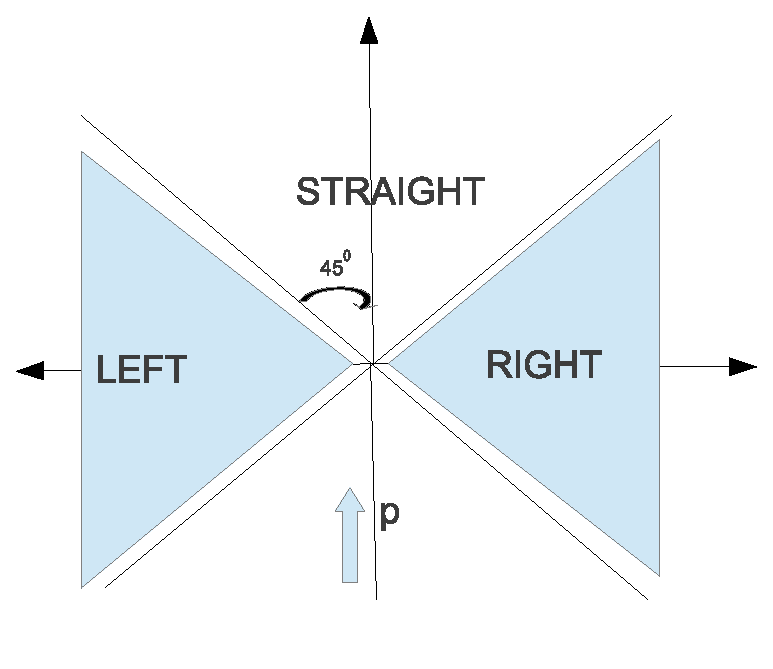
\epsfig{file=simpleturns.eps, height=3in, width=4in}
\caption{A decision point is simple intersection, if in each zone of the navigator's field view, there is atmost one road segment emerging from the decision point.}
\label{fig:simpleturns}
 \end{figure}
\subsection{Complex Intersections}
\begin{figure}
\centering
%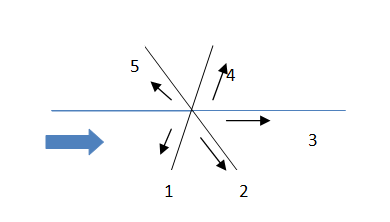
\includegraphics[width=0.5\textwidth]{complex.png}
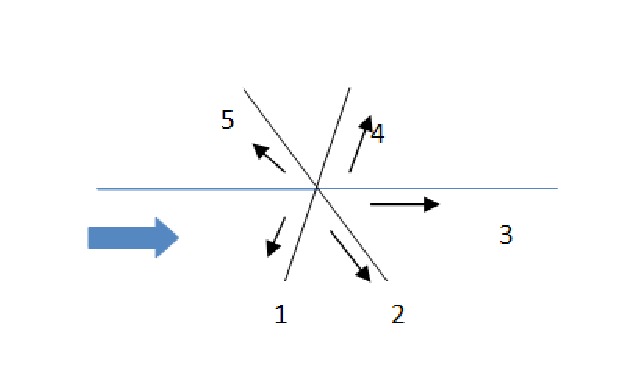
\epsfig{file=complex.eps, height=2.5in, width=5in}
\caption{Clock-based convention (anti-clockwise ordering) to non-ambigously represent directions at complex intersections}
\label{fig:complex}
 \end{figure}
\begin{figure}
\centering
%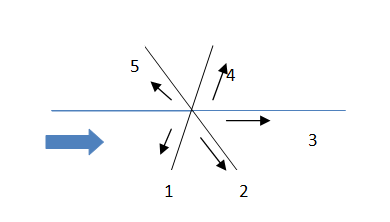
\includegraphics[width=0.5\textwidth]{complex.png}
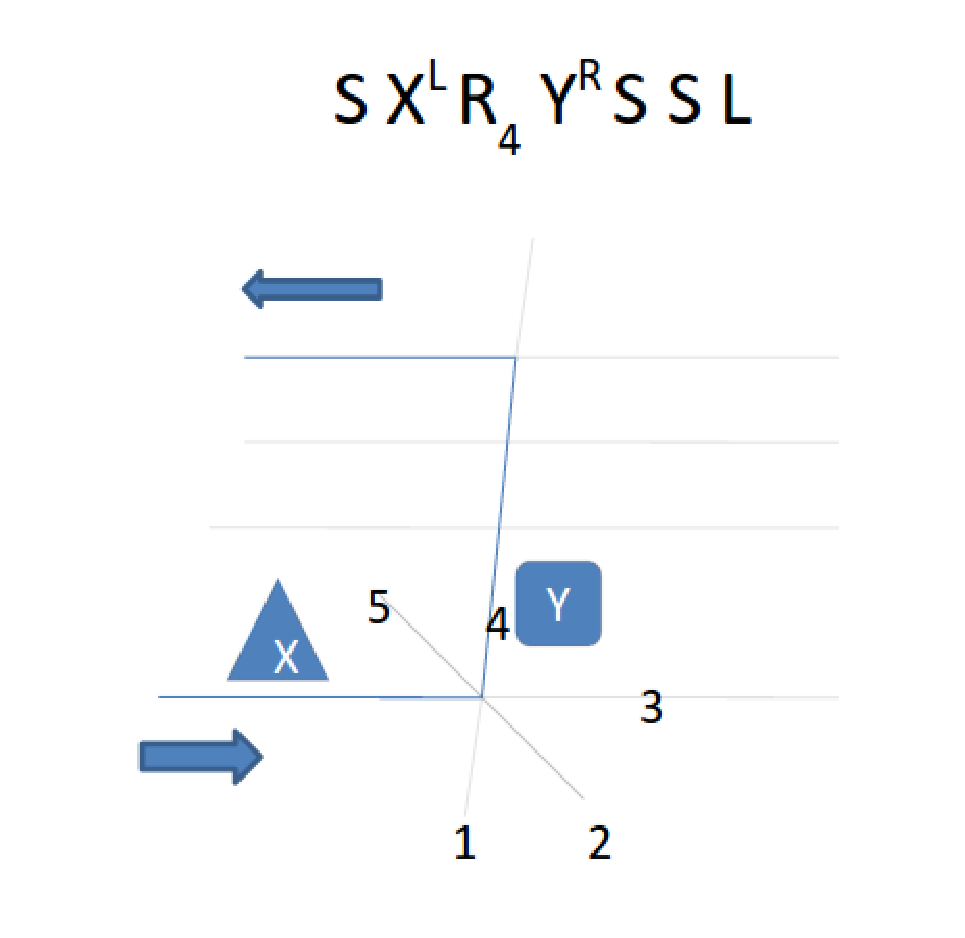
\epsfig{file=complexex.eps, height=3.5in, width=3in}
\caption{An example to showcase an application of the proposed 
communication protocol. The intended route is represented symbolically in 
text at the top of the image. One possible translation of the encoding in 
English can be as: 
1. \textit{Go Straight}
2. \textit{You would find X on your left}
3. \textit{At the intersection, take the 4th link in anti-clockwise direction from the most adjacent turn at your right side} 
4. \textit{You would find Y on your right}
5. \textit{Take the third left after Y}
}
\label{fig:complexex}
 \end{figure} 
Any decision point which is not a simple intersection is a 
\textit{complex intersection}\footnote{See Figure \ref{fig:complex_real} 
and Figure \ref{fig:complex}}. For representing complex intersections, we 
use a clock-based notation for a non-ambiguous representation. Klippel 
\cite{klippel} handles non-standard turns by using an 8-sector model which 
opens up alternate notations such as \textbf{hl} (half left), 
\textbf{vr} (veer right), etc. These work well for 4-way intersections 
and 3-way intersections but as the number of merged road segments 
increase beyond 4, the 8-sector model fails as there can be more than one 
road segment in the same sector. A clock-based notation does not work on the 
basis of a sector model and can handle extended multi-way intersections.

There are two ways to conceptualize a clock-based numbering scheme - clockwise and anti-clockwise. A user who is restricted to travel in a clockwise direction around a complex intersection has to be given instructions using the direction of travel as a reference. Thus, a fixed numbering scheme can not work in all scenarios. For example, in India, the direction of travel is clockwise, while in western countries it is anti-clockwise. Hence, we chose to specify whether the numbering is clockwise or anticlockwise at a global level and then let the algorithm make use of it. In the below discussion, we assume the global specifications pertaining to anti-clockwise direction of travel.

The roads are represented in an anti-clockwise numbering starting from the first turn right-adjacent to 
incoming road segment as shown in Figure \ref{fig:complex}. Notationally, 
we represent complex turns in the form $R_i$, which represents the 
$i^{th}$ numbered turn in an anti-clockwise direction starting from the most 
adjacent turn on your right.

Figure \ref{fig:complexex} elaborates a full-fledged example combining 
the representations of landmarks and intersections and attempts to 
present an english translation of the same. Before we conclude, we claim 
that the qualitative calculi used by Klippel \cite{klippel} on formal 
representations can be applied likewise to the proposed communication 
protocol as it directly extends it by including 
complex intersections. So if a route has no complex intersections, our 
communication protocol is semantically similar to that of Klippel. 
Continuing the example from Figure \ref{fig:complexex}, the route 
segment corresponding to the representation $SSL$ is translated as 
\textit{the third left} which is similar to the chunking rule of 
Klippel's \textit{wayfinding choremes} \cite{klippel}, where by the help 
of term rewriting, an intermediate representation is deduced from simple 
representations, prior to natural-language translation.

%We implemented this protocol and incorporated in our testbed to demonstrate the validity and non-ambiguity of its semantics.
 \chapter{Dialog-Based Localization}

In the previous chapter, we proposed a communication protocol to convey 
turn behaviour at every intersection. In this chapter, we introduce the 
algorithm for dialog-based tracking between intersections to 
determine an user's location and temporally align the delivery of route 
instructions with the user's movement and confirm his location and 
orientation. While posing questions to a user for localization and 
confirming orientation we propose alternative way to reference 
landmarks which highlights distinctive geometric features. We next 
present a method to extrapolate movements of a user for location 
inference using speed predictions. To further cope with errors and 
misinterpretations, we also introduce algorithms to detect and 
resolve disorientation. The localization alogrithm along with the 
communication protocol are the two mutually exclusive and exhaustive 
components of the proposed location-unaware dialog-system. 

\section{Introduction} 
While guiding a user to his next path segment, it is necessary to keep track 
of an user's location to avoid any disorientation. Since, there is no 
device-based support for location sensing, the only way to localize a 
user is by asking him about his location in a controlled input format. 
Though, researchers 
\cite{tellex:language, Kordjamshidi:labelling, matuszek:following} have 
been working on processing unrestricted NL input to extract spatial 
information but none of these have been able to overcome the classical 
information extraction errors limiting the output. Further limitations 
are imposed by poor speech recognition and the ineffectiveness of using 
unrestricted language as input.
 
For this work, we try to limit the questions to those with an objective 
reply (such as yes or no) or recognisable speech commands (such as color 
of a building, etc.). These questions are strategically based on the 
salient features of the spatial environment i.e. \textit{landmarks}. The 
other requirement to provide a quality user interface is to be able to 
predict the correct position of the user with reasonable precision, such that the number of questions asked to confirm the orientation and 
localize the user are kept to a minimum. The `number of questions asked', as 
we would discuss later in detail in Chapter \ref{evaluation}, is a 
prime evaluation criterion.

\section{Alternative Reference to Routemarks}
\label{sec:altref}
In any session of wayfinding, a user is incrementally guided for turn 
behavior at every intersection. Between every two intersections, a user is 
prompted for localization via questions based on whether he encountered 
the associated landmarks en-route\footnote{The issue of how landmarks 
are associated with a path segment is discussed in Section \ref{sec:kbase}.}. 
Lovelace et al. \cite{lovelace} distinguish between landmarks 
according to the purpose they serve i.e. either in choosing the action at 
a decision point (landmarks) or confirming reorientation on a path 
segment (\textit{routemarks}). In localization, landmarks are always 
treated as routemarks and with this, there is a difference in how they 
are communicated to the user. In the following discussion, the term 
landmark would be used substitutively for a routemark. 

A landmark is referred to by it's name (e.g., Eiffel tower) or by it's 
category (e.g., hospital, T-junction) or both, depending on whichever 
defines it's distinctiveness in it's locality. Although, in general 
category-based landmarks are easily comprehensible under route 
instructions but similar familiariaty is not guaranteed with name-based 
landmarks unless the name is explicitly mentioned in a readable form 
(like for hotels). In such cases, it is preferable to refer a landmark by 
it's distinctive geometry feature (if any or else choose a landmark by 
geometry). For example, instead of refering to that building as 
\textit{Visitor's Hostel}, the system should refer it alternatively as 
the ``red colored 2-floored building'' if it is the only one so in the 
locality. Since, even a category-based landmark can be misinterpreted, esp. 
when it's structure does not directly reflect it's category (like a movie 
theatre might not look like a theatre), we reference a routemark by it's 
distinctive geometry feature if it's salience falls below a certain 
threshold. The threshhold parameter differs for name-based landmarks 
based on the assumption that the chances of unfamiliarity to a name are 
more than the mismatch of landmark structure with it's category.
\section{Extrapolating User Movements}
\subsection{Estimating User Speed}
Consider a situation when the user is on a particular path segment and 
is being guided to his destination through an incremental set of 
instructions. At this point, the instruction pertaining to the next 
intersection has been made known. The prompts are such that the user is 
required to give a positive response only when he sees a particular 
landmark after taking the needed action. For example, a natural language 
equivalent (in English) of such a prompt could be, \textit{Go straight at 
the next intersection and prompt me `Yes' when you see a cafeteria on 
your left}. These instructions as discussed earlier are a part of the 
communication protocol. At this point, if the user follows the 
instruction correctly and takes a non-turning action at the next 
intersection, he should see the \textit{cafeteria} on his left after some 
point of time. Since, the instructions do not explicitly or implicitly 
mention any intersection in between, it is guaranteed that between 
the \textit{cafeteria} and current location of the user, there is exactly 
one intersection. The time when a positive response is recorded from the 
user, the \textit{cafeteria} becomes the new current location of the user.
Thus based on distance measures and the corresponding time difference, 
speed can be computed. Thus, speed estimation can be approximated  as:
\[\displaystyle \textit{User Speed}=\frac{\textit{Distance between two recorded prompts}}{\textit{Time difference between the two prompts}}\]
\subsection{Predicting User Speed}
\label{sect:predictspeed}
Speed predictions allow adaptive localization 
and help to extrapolate movement patterns of a user based on the speed 
profile. Continuing from the above example, consider a case when an user 
does not respond with a `Yes' prompt for a relatively long time. If the 
system acts passively waiting for the `Yes' prompt, a disoriented user 
may be totally lost (unless the system accepts unrestricted NL to process 
a general user query). Thus, there needs to be a predefined time limit within 
which the user is expected to provide a response. If this time limit 
expires, the sytem can interrupt to generate another prompt confirming 
his location/orientation. To get an estimate of this time limit it is 
necessary to predict the speed of the user. 

The speed predictions are specific to a road segment and time of day. 
Some roads allow faster speeds than others but the differences 
differ over the time of day.
Also to be considered is the speed profile of the user. A generally 
slow driver is likely to drive proportionately slowly in every speed-limit scenario. 
Summing up, the algorithm for speed prediction works over two predictors - 
\begin{itemize}
\item historical average speed on the road segment at this time of day 
$(H_{e,t})$,
\item average relative speed deviation of the user from the historical 
speeds $({A_u})$,
\item dynamic slowdown factor (f).
\end{itemize}

For every upcoming road segment, speed is estimated using the historical 
average speed on the road for the current time slot and the average 
deviation for the user in this session from the historical average speed 
on already travelled roads. 
The feature historical average speed is stored specific to discrete time 
slots in a day since a road might be distinctly fast at certain times of
the day for example in the late nights as compared to 
peak-hours. The average relative speed deviation feature is a
characteristic of the current user and can help identify driving preferences. 
This gives a slow driver a longer time gap between successive prompts for 
confirming orientation, while a fast driver might get quicker prompts 
to spatio-temporally match his rapid movements.  

The third predictor is meant to consider live traffic information. There 
may be cases when a road has a history of fast vehicle operating speeds and 
yet, temporary slowdowns maybe observed even for drivers with high-speed 
driving preferences. Such slowdowns can occur due to natural causes   
such as foggy weather or rain or snow. Some times the reasons can be man-made 
like festival celebrations, rallies or occassional traffic-jams. The 
estimation of the dynamic slowdown factor is 
done afresh in each time slot by averaging relative slowdowns
of all the users on the given edge/segment and can be modelled as:
\[\displaystyle f_{e} = \frac{1}{|U|}\sum_{u \text{ } \in \textit{ U}}(1-\frac{(A_u - A_{e,u})}{A_u})\]  
\begin{align*}
A_{e,u} - \text{speed deviation of user} \textit{ u } at \textit{ e } \text{from historical average speeds at }\textit{e} \text{ at given time slot} \\
A_u - \text{average relative speed deviation of the user \textit{u} from the historical average speeds} \\
U - \text{the set of users who travelled the edge \textit{e} in this time slot} \\
f_e - \text{slowdown factor for edge \textit{e} at given time slot}
\end{align*}
\section{Detecting Disorientation}
As discussed before, exactly one prompt is posed to the user between 
every two intersection points. For a road segment this prompt asks the 
user to confirm his position and is put out as early as possible 
to detect any disorientation earlier rather than later. When no response
is received within the time limit there are two cases (see 
algorithm below).  Algorithm \ref{algo:detect} presents the algorithm to 
detect disorientation.

\begin{algorithm}[H]
\label{algo:detect}
\SetVline
\dontprintsemicolon
\SetKwInOut{Input}{input}\SetKwInOut{Output}{output}
\Input{Response received at the end of time limit (can be None), \\the landmark position expected and\\ current time limit}
\Output{1, if detected disorientation, 0 otherwise}
\BlankLine

\eIf{response is positive}{
go to next route segment\;
current location becomes this landmark\;
}{
prompt to ask if the intermediate intersection was crossed\;
$response \leftarrow getInput()$  

\eIf{response is positive}{
    $timeFrame \leftarrow timeFrame\times waitFactor$\;
    \tcp{wait for timeFrame}
    $response \leftarrow getInput(timeFrame)$ \tcp{blocks for timeFrame units} 
    \eIf{response received and response is positive}
      {return 0\;}
     {
     \tcp{Here when no response received or negative response}
     return 1\;} 
  }
{return 0\;}
}
\caption{DetectDisorientation(response,landmark,timeFrame)}
\end{algorithm}
\subsection*{Case I - Slow Driver}
If the user is unable to reach the next position within the expected time 
frame, then he might not be able to see the instructed landmark before 
the end of the time limit and thus no `Yes' prompt would be received even 
though the user is not disoriented. Since, it is  possible to be 
slow in crossing an intersection especially if it involves traffic 
signals the system asks whether 
the intermediate intersection was crossed. If the answer is `No', then 
the system delegates the next position to this intermediate intersection 
and waits for a `Yes' prompt which if received, confirms that the user 
has crossed the intersection. 

\subsection*{Case II - Disoriented User}
However, if the system receives a `Yes' prompt at the inquiry for 
crossing the intersection, it waits for an additional time frame (a duration
equal to the original time frame reduced by a wait factor). This 
additional time frame is used to accomodate possible slowness of the 
driver assuming that the user though running a little slow would 
encounter the desired landmark at the next path segment. Once the 
additional time frame expires and still the user does not see the instructed 
landmark despite having crossed the intesection, the system assumes the
user is disoriented and works on reorienting the user.
This situation is depicted in Figure~\ref{fig:detect}. 
\begin{figure}
\centering
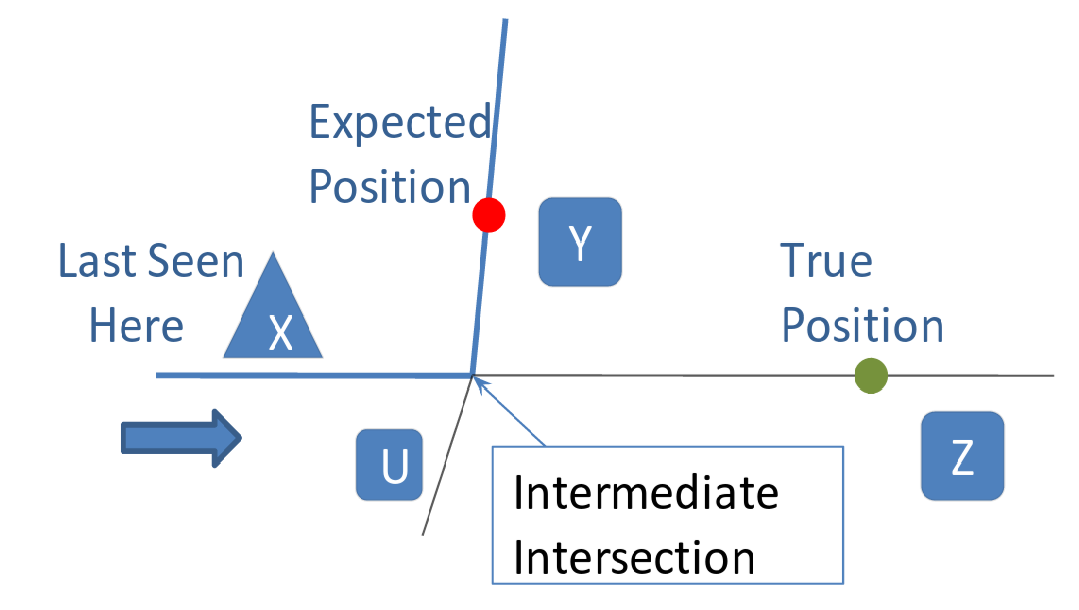
\epsfig{file=disorientation.eps, height=2in, width=3in}
\caption{\textbf{Detecting Disorientation} The highlighted route denotes 
the path segment communicated to the user for wayfinding. The user has 
strayed from the desired path segment and has been detected by the 
system after a positive response on querying on whether the intermediate 
intersection was crossed.}
\label{fig:detect}
 \end{figure}
\section{Reorientation algorithm}
\label{sec:reorient}
The process of tackling disorientation is divided into two phases, each 
with it's own characteristic way of causing reorientation. 
\subsection*{Phase I: Anticipative}
The first phase is an \textit{anticipative phase} where user's position is estimated based on movement extrapolation using all possible paths from 
the last seen point (LSP). The idea is to localize the user to the 
nearest landmark visited by the user. In the act of localization, the 
user is prompted with the possible landmarks he could have encountered 
en-route. For example, consider the case shown in Figure 
\ref{fig:anticipative}. Once disorientation is detected for the user, 
based on speed predictions, the possible path 
segments and associated landmarks are identified. Thereafter,  
the user is prompted with questions identifying these landmarks (\textit{U, V, W} 
\textit{Z}) along with the orientations w.r.t. the user (left or right) to 
estimate his location. Reorientation is achieved when the user 
acknowledges any of the identities put in the prompts.
\begin{figure}
\centering
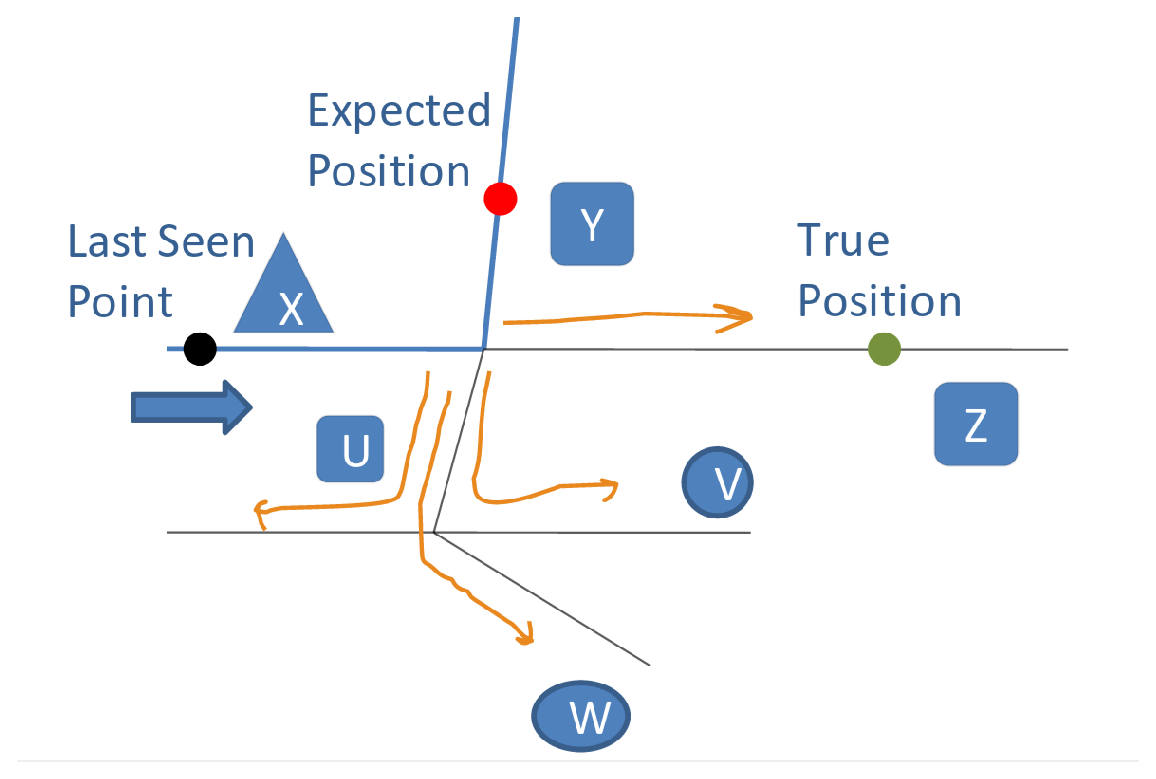
\epsfig{file=reorientationAnticipative.eps, height=2.5in, width=4in}
\caption{\textbf{Reorientation:Anticipative-Phase} Prompt the user with 
questions identifying landmarks \textit{U, V, W} and \textit{Z} along 
with the orientations w.r.t. user (left or right) to estimate location. 
Reorientation is achieved when the user acknowledges any of the 
identities put in the prompts.}
\label{fig:anticipative}
 \end{figure}
\subsection*{Phase II: Reactive}
When a small number of prompts suffice to reorient the user one can 
directly query for the identities of all landmarks seen on the way.
But when the number of prompts goes beyond an acceptable level
we opt to switch the reorientation strategy. Until now, the strategy was 
to be anticipative and the questions asked were of the form `\textit{do 
you see U on your right?}'. In the reactive strategy, an attempt is made to 
capture the environment of the user by querying over well-defined 
attributes. For example, the prompts now are of the form `\textit{do 
you see any building nearby?}' The term `\textit{building}' here is one 
of the categorizing attributes of landmarks which is a part of the 
feature-set stored as visual features in the knowledge base\footnote{See Section \ref{sec:kbase} for more details}. The feature-set 
includes attributes like color of the buildings, heights, shapes of the 
open spaces and other automatically extractable attributes.

The major drawback in solely relying upon the above strategy is that it 
does not guarantee localization. The approach is dependent on the stored 
visual features. In some cases, even after exhaustively asking questions 
on the categorizing attributes, there might still remain a set of possible 
locations the algorithm has not considered. For example, in a 
homogenous neighborhood the buildings in all the streets might look alike in 
shape, color and height. In such cases, when there are still a set of 
locations under consideration, the user is asked to continue his movement 
only to be interrupted later for yet another reorientation. This process is
iteratively repeated until the responses resolve the location of the user uniquely.

The reactive approach is analogous to \textit{scene analytic} 
location sensing techniques \cite{hightower}. These techniques work on 
visual images or electromagnetic measurements to sense observed features 
of a scene for determining a user's physical location. Understandably, 
the features used are those that are easy to represent and compare from 
an observed scene. The approach mentioned is a hybrid of \textit{static} 
and \textit{differential} scene analysis. In the former technique, the
features in question are looked up in a pre-defined geo-spatial database, 
whereas in the latter, differences in scenes observed due to an user's 
movements are used to match known spatial environments.

 \chapter{Implementation}
 \label{chap:implement}
In Chapter \ref{chap:concept}, we discussed the 
architecture of a generic wayfinding model and the structure and interaction 
of the different modules. This chapter describes the implementation-specific 
aspects of the key components. We discuss a methodology to build the 
knowledge-base by automated extraction of attribute-values and 
identification of associations with corresponding entities to 
represent spatial information. Furthermore, for reorientation, 
we introduce our approach to study movement patterns in order to 
facilitate early localization of a disoriented user.

 \section{Knowledge Base}
  \label{sec:kbase}
\subsection{Extracting Attribute Values}
Raubal and Winter \cite{raubal} in similar research categorized
the attributes defining landmarks and provided a methodology to 
automatically extract local landmarks using integrated datasets such as a
3-D city model, navigation graphs and georeferenced images of every house 
in the neighbourhood. Such an approach offers resources to populate the 
visual and semantic attributes. But, they also say that to extract 
visual and semantic features, one needs comprehensive datasets and 
extrinsic dependence.  Brenner and Elias \cite{brenner} focussed on 
extracting landmarks structurally using data mining on spatial 
databases. The approach focusses more on intrinsic attributes (such as 
form factor of a building, distance off the road segment), values 
which are extractable by processing the map itself. They also 
highlight the use of laser methods to identify certain visual features 
(such as height, visibility).  The various attributes considered in their 
work to extract salient landmarks are shown in Figure \ref{fig:elias}.

We opted to work on the lines similar to \cite{brenner} to define the 
geometric salience of buildings. In a real-world application, only those 
attributes should be considered that are identifiable and communicable. 
For example, \textit{form of parcel} (in Figure \ref{fig:elias}) might be 
a difficult attribute to realize in English language and equally 
difficult to be identified by a driver. On the other hand, \textit{road 
distance} is easily identifiable and communicable. Apart from the 
buildings, we also considered open spaces (such as playgrounds or parks) 
while searching for salient features in a neighborhood. Though a street 
may well be surrounded by structurally similar buildings but a large 
enough open-space area in it would be sufficient to confirm orientation 
of the user if there is no such feature in the neighbouring streets. We 
do not rely upon the visual and semantic attributes of a landmark for two 
reasons: (a) the geodatasets used for extracting such information are 
scarce and limited, and (b) the requirement of our guidance algorithm 
from the attributes of a landmark is fulfilled if they can make the 
landmark uniquely identifiable in it's local neighborhood. Though visual 
and semantic attributes would enhance the identifiability but the 
algorithm is adaptive to the absence of such attributes. We tested the 
usage of such attributes in guidance and localization using synthetic 
settings wherein the number of available attributes was parametrized and 
attribute values were randomly assigned.

\begin{figure}
\centering
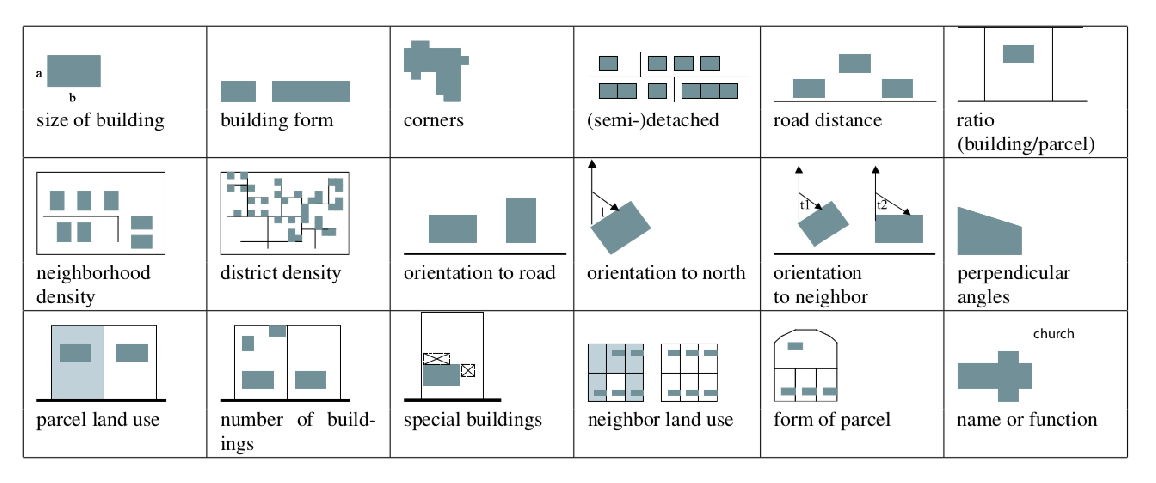
\epsfig{file=brenner.eps, height=2in, width=6in}
\caption{\textbf{Extracting Geometric Salience} The geometric attributes 
used by Brenner and Elias \cite{brenner} to extract building-based 
landmarks}
\label{fig:elias}
 \end{figure}

Semantic attributes pose a challenge for automated extraction and demand 
sophisticated web-mining approaches for qualitative results. Tezuka 
and Tanaka~\cite{tezuka} present one such approach of exploiting the
web to extract landmarks from digital documents with good precision. 
However for the purpose of this work, we used a simple and scalable 
approach to extract the semantic attribute of \textit{popularity} using web 
resources in order to enhance feature identifiability wherever possible. 
The popularity of a landmark can help in deducing familiarity of a 
navigator\footnote{Also, see Section \ref{sec:altref}}. For example, if a 
user comprehends instructions which refer to less popular landmarks by 
name, it can be assumed that he is familiar with the neighborhood 
and thus, instead of using geometric features for making a landmark 
identifiable, the local names of the landmark can be used for wayfinding 
assistance. The extraction methodology\footnote{Depicted in Figure \ref{fig:popular}}
 exploits two well-known mapping applications as resources: Google Maps \cite{gmaps} and Wikimapia 
\cite{wiki} and is described below.  Also, since these applications also collect metadata in 
the form of user reviews, they can be utilized to obtain local names/aliases 
for the spatial features of an environment which are not present in 
traditional geodatabases.
\subsubsection*{Using Google Maps}
To help provide development services, Google-Maps provides a ranking 
scheme to search for popular places in a nearby area via it's Places API. 
The ranking scheme utilizes the quality of citations and reviews to 
places done by it's large user base. The search results show 
upto 60 places ranked in the order of prominence for a given query for a 
given radius. Thus it forms a convenient application to find popular 
places in a neighborhood or equivalently to find popularity of a given 
location as compared to others in it's local neighborhood. We applied this 
methodology to the IIT Kanpur campus and used the results of the search to 
contribute to the \textit{popularity} attribute. Due to a comparatively 
small area occupied by the campus, the attributes were populated with a 
single search query with radius set to 2km from PK Kelkar Library, the 
approximate center of IITK campus.

\subsubsection*{Using Wikimapia}
Unlike Google Maps, wikimapia is an open-content mapping application and 
it provides free access to it's extensive geodatabase. The maps in 
wikimapia are edited and updated via crowdsourcing. And, unlike 
Google, it does not provide a ranking index to directly find the 
prominence of a location. But, it does provide open access to all the 
reviews submitted for the places in it's spatial database. Based on the 
heuristic that a popular place would have a comparatively large number of 
reviews submitted, we extract and map popularity to the corresponding 
locations using the number of reviews as an index. Under wikimapia, we 
define popularity of an area as the total number of reviews of 
all places within it.
\begin{figure}
\centering
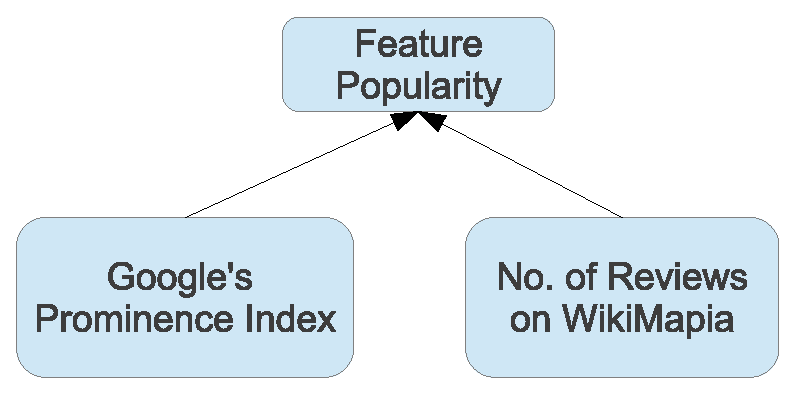
\epsfig{file=popular.eps, height=1.5in, width=2in}
\caption{\textbf{\textbf{Extracting Popularity}} A scalable approach to 
get an estimate of the popularity of a landmark using 
mapping applications.}
\label{fig:popular}
 \end{figure}

\subsection{Identifying associations}
Having combined resources for extracting attribute values for creating 
relations for the features of an environment, the need is to provide an 
interface to use this spatial information in a real-time wayfinding 
assistance task. To be able to use the features in route instructions, 
every road segment needs to be associated with a certain feature (landmark) 
which serves to confirm the orientation of a user. For the purpose of 
this work, we used a nearness heuristic based on the closest distance 
between the landmark and the road to identify the association between a 
landmark and a road segment. The distance thresholds qualifying a 
landmark's association are chosen to be minimum so as to allow 
identifiablity of attributes by a driver. 

If visibility analysis methods are available (3D models, laser scanning, 
etc), distance criteria cannot be relaxed beyond a certain point since even
though a landmark is visible from the road there is no guarantee
that the attributes of the landmark can be identified by a 
distant driver. Also, as per Lynch \cite{lynch}, distant landmarks are 
used only for overall guidance for novice users.

\section{Facilitating Reorientation}
\subsection{Anticipative Phase}
\label{sect:anticip}
In Section \ref{sec:reorient}, we discussed the algorithm to reorient a 
disoriented user by querying over possible paths. Trajectory predictions 
can assist in reorientation by studying distraction patterns which can be 
exploited for faster localization. These patterns may arise due to 
environmental factors, complexity of the underlying communication 
protocol or arbitrary human errors. Trajectory prediction algorithms have 
been previously developed for improving QoS in cellular mobile networks 
\cite{kyri} and facilitating location based services by predicting 
future locations \cite{karimi}. These situations differ from the 
context of disorientation in wayfinding in which the movements are 
based on route instructions. 

Here, we propose an approach for trajectory prediction based on probabilistic 
modelling of movement under the constraint of route-instructions and 
extends the constraint-free modelling approach adopted in \cite{liu}. The 
model calculates the probability of disorientation on a particular road segment 
($Y$) from the given path segments ($X,I$). To realize the model, the 
required probability is output from a conditional probability $P(Y|X,I)$ 
which can be written as:
%
$$D_{S_1,R_1,R_2} = P(Y=S_1|X=R_1,I=R_2)$$
%
where $S_1,R_1$ and $R_2$ are road segments and $D_{S_1,R_1,R_2}$ is the 
probability of choosing road segment $S_1$ when the user is currently 
on $R_1$ and instructed to move next to $R_2$. The probability is 
estimated based on historical movement patterns and can be formulated as
%
\[ \displaystyle P(Y|X,I) = \frac{N(Y|X,I)}{ \mathlarger{\sum}\limits_{y \in O_{X,I}} N(y|X,I)} \] 
%
where $O_{X,I}$ is the set of all the road segments at the intersection 
of $X$ and $I$, and $N(y|X,I)$ is the number of times road segment $y$ 
has been taken from $X$ when the next instruction was to take $I$. 

Thus, the reorientation algorithm sorts the road segments in decreasing order 
of probability to disorient to, and prompts them incrementally to the 
user until a positive acknowledgement is received or limit to the number 
of prompts is exceeded after which it enters into reactive phase.

\subsection{Reactive Phase}
While reorientation is facilitated in anticipative phase through probability modelling, in reactive phase, we use entropy measures to identify the odering of questions to be posed to the user. Since reactive phase deals with questions based directly on the attribute-value pair of the landmarks surrounding the user's location (e.g., \textit{do you see a white-colored building around you?}), it is important to identify the most informative pair knowing the response to which maximally prunes the search space. This problem is similar to the machine learning problem of structuring a decision tree, where the most informative attribute-value pairs are identified and placed at the top of the decision tree. Such a structuring yields the preferred sequence of attributes to inquire, to most rapidly narrow down the class of an entity. 

The methodology used to identify the preferred sequence of attributes to inquire is defined below:

Suppose, the set of road-segments suspected for location of the user is $X$. Corresponding to each of these segments, we identify the associated landmarks and collect them into a set $L$. Thus, $L$ is a set of potential landmarks visible to the user at this particular time. Each landmarks $l$ in $L$ has a certain set of attributes, values $V_{l}$ of which may overlap amongst more than one landmark (for example, there may be multiple \textit{red colored} buildings in the locality). The problem is to identify the attribute-value pair which helps prune the possible locations of the user by a good enough extent. The problem is broken down into two steps- 1) identify the attribute to inquire for and, 2) identify the value of this attribute to inquire, to output the preferred attribute-value pair. 

\subsubsection*{Identifying the best attribute}
 To identify the best attribute from the set of attributes, we first define entropy $E_a$ of an attribute $a$ as follows:
\[\displaystyle E_{a} = - \sum_{v \in V_{a}}f_vlog_{2}{(f_v)}\] 
where, \\
$V_{a}$ is the set of values for attribute $a$ and, \\
$f_{v}$ is the ratio of elements in $L$ with the $v$ as the value of attribute $a$.

It can be observed that $E_a$ is 0, when all landmarks have the same value for attribute $a$. Inquiring upon such an attribute to the user does not lead to any pruning and is thus the least preferred attribute. $E_a$ is maximum when the values of $a$ are almost equally shared in all the landmarks. In this case, based on a response to the question asked upon the value of attribute $a$, more locations can be pruned off. Thus, the most preferred attribute to inquire is the one which has the maximum entropy.

Hence, the equation for finding the best attribute $a_{opt}$ can be defined as below:
\[\displaystyle a_{opt} = \operatorname*{arg\,max}_a E_a\] 

\subsubsection*{Identifying the best value}
Finding the best attribute is not sufficient for the cause of building a dialog-based system ensuring simple speech processing. It is preferable to limit the response of the user to an objective one rather than something subjective which demands qualitative speech processing requirements. For example, it is preferable to ask a question like, `do you see a red colored building nearby?', rather than something like, 'what is the color of building you see?'.

The same entropy rule applies to finding the best value only that entropy of a value ($E_v$) differs from the definition of an attribute and, is defined below:
\[\displaystyle E_{v} = - f_vlog_{2}{(f_v)} - (1-f_v)log_{2}{(1-f_v)}\] 

 \chapter{Evaluation}
This chapter describes an intrinsic evaluation of our proposed model, 
particularly focussing on the ability to localize and reorient a 
disoriented user. The evaluation is conducted by modelling user behavior 
with paramters to characterize speed profile and erroneous behaviour. We 
then measure the performance of the guidance algorithm under a dialog-
based interface with regards to quality of user experience. To our 
knowledge, there has not been any previous work using a virtual user 
model for evaluating wayfinding guidance. 
 
 \label{evaluation}
 \section{Dataset}
We begin by describing the dataset for our prototype implementation. The 
dataset used for implementation of the model was taken from the 
geospatial data of Indian Institute of Technology, Kanpur (IITK). The raw 
data consists of shapefiles representing different layers of a GIS 
including road network, geometry and metadata of spatial features such as 
academic buildings, residential areas, parks. Visually, the IITK 
environment depicts a mix of regions which are variably dense in terms of 
landmark density (Figure \ref{fig:dataset}). On one hand, the academic 
area is filled with a plethora of distinct features which can be easily 
identified by an unfamiliar navigator on the other hand residential 
regions have almost no salient landmark or mutually distinguishing 
features except for unique house numbers. The 
academic area is built on a dense street network while there are long and 
clear demarcations in the residential areas\footnote{Prior to building the knowledge base preliminary processing 
is done on the road network data. Since the shapefiles for the road network 
are in raw geo-vector format, they need to be converted to a routable 
network for route computations. The road segments are split at 
intersections to create disjoint edges, each with a start and an end node.}.
\begin{figure}
\centering
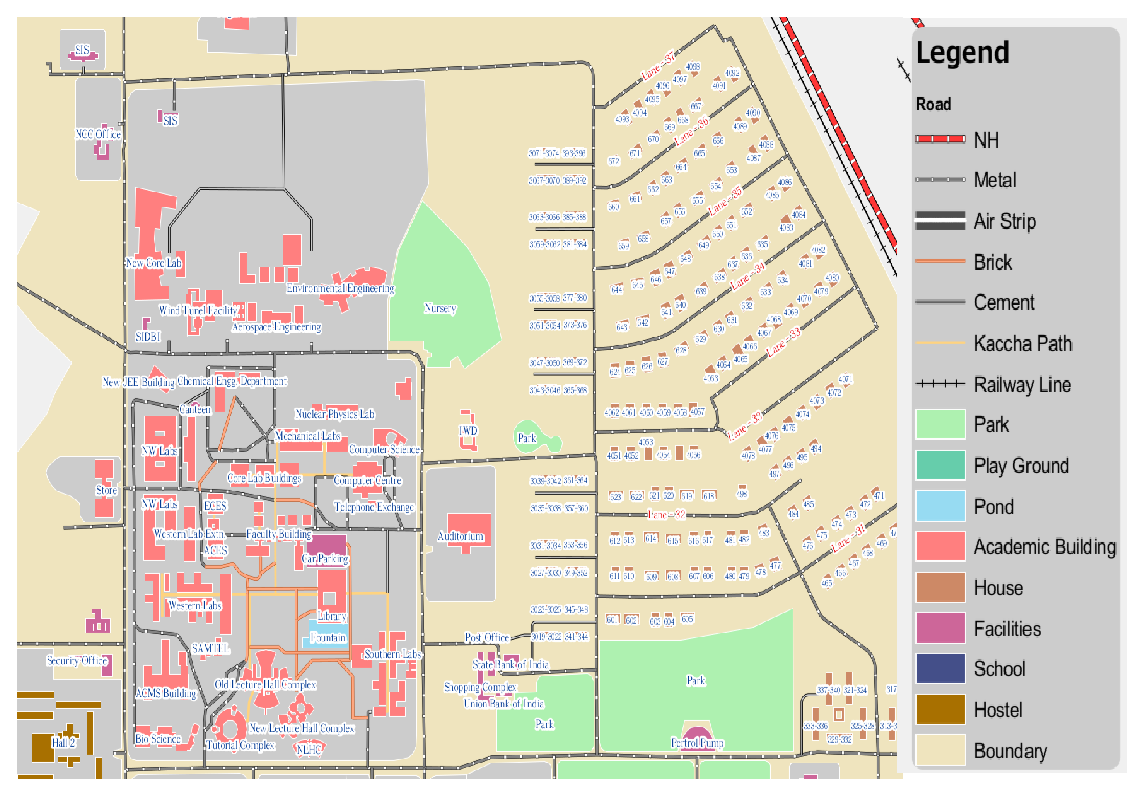
\epsfig{file=iitkmap.eps, height=6in, width=9in, angle=90}
\caption{\textbf{\textbf{Dataset}} Snapshot of a map of Indian 
Institute of Technology, Kanpur (IITK). The bottom portion of the snapshot 
depicting academic buildings (see legend) represents the landmark-dense 
portion of the campus, Academic area. The organized homogenous space to 
the top of it represents a portion of the residential areas which has 
no salient features.}
\label{fig:dataset}
 \end{figure} 

 \section{Simulation Setup} 
The time spent in executing real-time wayfinding tasks with actual
users limits the scope 
for comprehensive testing of a wayfinding-assistance framework. Furthermore,
simulations help in situation modelling which is vitally important in 
studying different scenarios of disorientation. The simulation rests on a 
virtual user model and a synthetic set of feature attributes. The user model 
simulates varying speed patterns with regard to human behaviour, while 
the synthetic attribute-set models the extent of diversity in spatial 
environments.
  \subsection{User Modelling}
  \subsubsection*{Speed Profiles}
The speed of a driver at a given road segment can be modelled using two 
parameters- 1) \textit{categorical-speed} (\textit{s}) parameter, to represent the 
speed preferences of a driver and, 2) \textit{deviation} (\textit{d}) parameter, to 
add an element of non-uniformity w.r.t the category to reflect individual
variations.

%The categorical-speed parameter of a driver is high for users with fast driving preferences and low for those with slow driving preferences. 
The categorical-speed for a driver is picked from a continuous 
probability distribution model. Previous studies \cite{leong,mclean}
have found the normal distribution to work under homogenous traffic flow 
(same type of vehicles) with moderate to low traffic volume conditions. 
However under heterogenous traffic conditions, researchers have proposed 
using a log–normal distribution \cite{gerl} for traffic modelling. 
The parameters of the distributions ($\mu= 2.7$, $\sigma=0.5$) are set such 
that the 85th percentile speed is equal to 25 kph i.e. the speed limit in 
IITK campus\footnote{This is in accordance with the observed relationship 
between vehicle operating speeds and posted speed limits.}. The 
deviation parameter can be sampled at each road segment from a normal 
distribution using categorical speed ($\mu=0$ kph, $\sigma=0.1\times s$ kph) and added to the 
categorical-speed to generate observed average speed at the road 
segment. However, for the purpose of this evaluation, we used uniform average speed modelling. This is because dealing with non-uniform speed models requires speed predictions which work only when there are definite patterns as in real-world traffic, else the results are inconclusive.
  \subsubsection*{Erroneous Behaviour}
To introduce disorientation in the model we use 
a simple error-making probability model for a user which governs user-behaviour at every decision point. One such very simple model is
where at an intersection the user chooses each segment at 
the intersection (except the one in use) with uniform 
probability. A more sophisticated error-making model would bias decisions 
based on the structure of the intersection. For instance, one may assign 
higher probability to go straight when asked to turn left (or right). 
This may be particularly useful in complex intersections where the 
probability for choosing a wrong segment is higher. 
  \subsection{Synthetic Attributes}
We discussed possible approaches to extract attributes of a spatial 
feature in Section \ref{sec:kbase}.  Since the focus of this 
work was on dialog-based localization, we chose to synthetically populate 
the attribute-set of the features. The number of attributes was 
paramterized in the testbed and the corresponding values were assigned 
randomly from a fixed set. The idea was to study how performance of the 
localization algorithm depends on the presence of extrinsic attributes. 
 \section{Goodness Metric}
The major concern with any wayfinding assistance is the extent of 
interference it causes to the wayfinder. Thus, quality of user experience 
in a dialog-based wayfinding system would heavily depend on the 
number of prompts required while assisting the user. As the complexity of 
a route increases in terms of the number of decisions to be made en-route, 
greater is the number of prompts required. Also, if a user 
commits an error in following the route instructions and is disoriented
additional prompts are needed to reorient the user. 

Based on the above discussion, we define a \textit{goodness} metric for the 
evaluation of the proposed model as the number of prompts 
needed by a user ($N_p$) normalized by the total number of decisions 
made ($N_D$) and the total number of disorientations ($N_e$) recorded 
before reaching the destination. The goodness metric ($G$) is defined 
as: 
\[\displaystyle G = \frac{N_p - \alpha \times N_D}{N_e}\]  
where $\alpha$ is a constant, representing the number of prompts made in 
guiding a user on a route with exactly one decision point.
 \section{Results} 
In this section, we describe the results obtained on running the 
simulations with an artifical agent whose behaviour is directed 
by the above models.
Before we present the results of the simulations, we describe below the 
assumptions made while programming the simulations:
 \begin{enumerate}
   \item The localization is done on a road-segment\footnote{A road 
segment is an atomic portion of the road with decision points
only on either end.} basis and we assume that 
localization was successful if the tracker correctly identifies the 
current road segment of the agent.
   \item The agent has perfect vision and correctly describes what he 
sees and what he does not see in his spatial environment.
   \item The agent can move along on any road-segment present in the 
network. 
 \end{enumerate}
 \subsection*{Anticipative Phase}
The first set of results report the average goodness metric ($G_{avg}$) 
using only anticipative reorientation (see Section 
\ref{sec:reorient}). This expectedly raises 
the number of prompts to alarmingly large and impractical values. 
Although, in an alternate strategy where a negative response (to 
a question on seeing a landmark) is attributed to the slowness of the user 
rather than a disorientation resulted in a substantial decrease in the 
number of prompts.  The results are summarized in Table \ref{table:st}.
\begin{table}[h]
\center
\begin{tabular}{|c|c|}
\hline
\textbf{Strategy} & $G_{avg}$ \\ \hline
1 & 16.8 \\ \hline
2 & 9.4\\ \hline
\end{tabular}
\caption{Strategy 2 accommodates slowness of the user and extends a naive strategy (Strategy 1) by waiting longer instead of suspecting disorientation and results in a substantial decrease in number of prompts.}
\label{table:st}
\end{table}
\subsection*{Reactive Phase}
For evaluating the reactive phase, we need queries over the attributes of 
a landmark, which for the purpose of the evaluation were synthetically 
created. Here, we studied how many attributes will be sufficient 
for successful dialog-based localization. The idea is that if the 
number of attributes required for localization is not very large, 
intrinsic attributes should be enough to serve the need of referring to 
landmarks.

From the performance of the model on the simulations using purely reactive phase of reorientation, it was observed that not always it is possible to localize a user by asking questions from his spatial environment. This is understandable because if the features in an environment don't differ much from each other, it is hard to distinguish one locality from the other based on the attributes alone. However, the advantage of using reactive phase is that the number of questions asked to localize a user (possibly disoriented) is significantly smaller than that of anticipative phase. The results on the synthetic dataset indicate that the number of successful localizations (or reorientation) increases with the number of attributes, while the number of questions asked increase only marginally, and are presented in Table \ref{table:att}. It was also observed that increasing the number of attributes beyond five does not substantially help in increasing the number of successful localizations. 
\begin{table}[h]
\center
\begin{tabular}{|c|c|c|c|}
\hline
              &                                                             & \multicolumn{2}{c|}{\begin{tabular}[c]{@{}c@{}}average number of\\ questions asked\end{tabular}} \\ \cline{3-4} 
\# attributes & \begin{tabular}[c]{@{}c@{}}success\\ rate (\%)\end{tabular} & \begin{tabular}[c]{@{}c@{}}positive\\ cases\end{tabular}                & overall                \\ \hline
1             & 43.24                                                       & 1.28                                                                    & 1.68                   \\ \hline
2             & 49.33                                                       & 1.40                                                                    & 2.10                   \\ \hline
3             & 62.5                                                        & 1.72                                                                    & 2.27                   \\ \hline
4             & 67.7                                                        & 1.55                                                                    & 2.12                   \\ \hline
5             & 69.7                                                        & 1.88                                                                    & 2.36                   \\ \hline
\end{tabular}
\caption{The number of successful localizations (or reorientations) increases with the number of attributes, while the number of questions asked increase marginally. The results of each attribute are based on 50 simulations of guiding an artificial agent for the same source and destination, modelling landmarks each time with a different attribute-set.}
\label{table:att}
\end{table}
The results obtained suggest that though the reactive phase leads to a 
significant decrease in the number of prompts, it does not guarantee 
localization. The anticipative phase on the 
other hand, leads to comparatively larger number of prompts but ensures 
localization (if the user is stopped when asking questions). The other 
advantage observed when working with the anticipative phase is that it 
imposes less cognitive load and/or distraction on the user as compared to 
the reactive phase. The questions in the anticipative phase are very 
specific to the spatial environment (e.g., \textit{do you see X on your 
right?}) and demand comparatively less cognitive processing than the
reactive phase (e.g., \textit{do you see a 3-storied building nearby?}). 

The implication drawn from the above results points towards a hybrid 
strategy combining anticipative and reactive components. As proposed earlier
(in Section \ref{sec:reorient}), the key is to limit the number of 
questions asked in the anticipative phase to an acceptable extent and then 
switch to the reactive phase. The reactive phase fails only when the 
landmarks do not have distinguishing attributes thereby creating ambiguity in 
possible locations of the user. Though, one cannot guarantee localization 
there are a couple of work-arounds to deal with it- a) when a 
reorientation attempt fails instruct the user to keep moving in a 
particular direction for a short while before being re-interrupted for 
reorientation and, b) link consecutive failed attempts to localize 
so as to prune possible positions of the user. 
 
 \chapter{Conclusion and Future Work}
This work presents the first attempt to a dialog-based wayfinding model independent of support for location-sensing or web-connectivity at the end-device. Such an approach is the only solution for providing wayfinding-assistance service to a person using vanilla end-device which can not render graphics or determine/send location information. 

This approach is different from other existing wayfinding-assistance 
models which use name-based reference to landmarks. We exploit the
idea that though a landmark may be salient due to its visual and geometric 
attributes it may be not be familiar by name. So,
the task of enriching route instructions with landmarks needs to consider 
the direct use of these salient attributes if the landmark in question 
is to be recognized by the user. 


We introduced a cross-lingual non-ambiguous representation of route instructions using simple formal language which can be easily translated to any desired natural language. The formal language extends the previous similar work by accommodating complex intersections into the language structure.

We take into consideration the issue of disorientation while guiding a user by using spoken-dialog conversations which is designed so as to overcome the limitations of speech recognition by ensuring questions are posed in a format which invoke objective replies, convenient to automated voice recognition.

We also present a unique approach for an automated evaluation of the quality of service of the model using a simulated set-up which models navigation behaviour of an artificial agent. The results indicate that by an appropriate mix of strategies of reorientation, a qualitative sytem can be built for dialog-based wayfinding using attributes of landmarks.

Our attempt to understand the challenges behind a location-unaware model for dialog-based wayfinding exposes several gaps in this research area. The significant differences achieved by changing strategies for reorientation motivate the search for alternate strategies to improve quality of service. The existing implementation can be directly extended to achieve better performance in terms of quality of service. In our implementation, on a failed localization, the user was instructed to keep moving foward, but no restrictions were enforced. The user would be interrupted later for another localization attempt but deductions from the previous failed localizations were not exploited henceforth. Further, speed prediction and probability-modelling for identifying movement patterns was not employed as it offers no support in artifical agents with random erroneous behavior. But in real-world scenarios, there are definite traffic patterns and the predictors mentioned in Section \ref{sect:predictspeed} and probability model discussed in \ref{sect:anticip} would be worthwhile to adopt. The evaluation of utility of these predictors can be studied by encoding patterns in the navigation behaviour of the artificial agents.  
 
\bibliographystyle{plain}
\bibliography{references}
%\addcontents{toc}{bibliography}
\end{document}
